\documentclass[12pt,a4paper]{article}
\usepackage[utf8]{vietnam}
\usepackage{amsmath,amssymb}
\usepackage{tabularx}
\usepackage{tikz}
\usetikzlibrary{calc,angles,quotes,arrows.meta,patterns}
\usepackage{xcolor}
\usepackage{enumitem}
\usepackage{fancyhdr}
\usepackage{graphicx}
\usepackage[top=0.9cm, bottom=0.9cm, left=1.2cm, right=1.2cm]{geometry}
\usepackage[loigiai]{ex_test}
\SAOPTN{widthSA=3.2,heightSA=0.62}

\setlength{\headheight}{15pt}
\setlength{\parskip}{0pt}

\pagestyle{fancy}
\fancyhf{}
\rhead{\textit{Môn Toán 8 -- Hướng dẫn giải Đề số 04}}
\lhead{\textit{Bộ đề ôn tập Giữa học kì I}}
\cfoot{\thepage}

\begin{document}

\begin{center}
  \textbf{\Large HƯỚNG DẪN GIẢI CHI TIẾT VÀ BẢNG ĐÁP ÁN}\\
  \textbf{\large ĐỀ ÔN TẬP GIỮA HỌC KỲ I -- ĐỀ SỐ 04}\\
  \textit{Môn: Toán 8 -- Năm học 2026 -- 2027}
\end{center}
\vspace{2mm}

% --- BẢNG ĐÁP ÁN TRẮC NGHIỆM TÓM TẮT ---
\noindent\textbf{\large A. BẢNG ĐÁP ÁN TRẮC NGHIỆM TỔNG HỢP}
\vspace{1mm}

\noindent\textbf{1. Phần I (Mỗi câu trả lời đúng được 0,25 điểm):}
\begin{center}
\begin{tabular}{|c|c|c|c|c|c|c|c|c|c|c|c|c|}
\hline
\textbf{Câu} & \textbf{1} & \textbf{2} & \textbf{3} & \textbf{4} & \textbf{5} & \textbf{6} & \textbf{7} & \textbf{8} & \textbf{9} & \textbf{10} & \textbf{11} & \textbf{12} \\
\hline
\textbf{Đ/A} & \textbf{A} & \textbf{B} & \textbf{B} & \textbf{B} & \textbf{A} & \textbf{A} & \textbf{C} & \textbf{B} & \textbf{A} & \textbf{C} & \textbf{B} & \textbf{B} \\
\hline
\end{tabular}
\end{center}
\vspace{0.5mm}

\noindent\textbf{2. Phần II (Đúng 1 ý: 0,1đ; 2 ý: 0,25đ; 3 ý: 0,5đ; 4 ý: 1,0đ):}
\begin{center}
\begin{tabular}{|c|c|c|c|c||c|c|c|c|c|}
\hline
\textbf{Câu} & \textbf{a)} & \textbf{b)} & \textbf{c)} & \textbf{d)} & \textbf{Câu} & \textbf{a)} & \textbf{b)} & \textbf{c)} & \textbf{d)} \\
\hline
\textbf{Câu 1} & \textbf{Đ} & \textbf{Đ} & \textbf{Đ} & \textbf{S} & \textbf{Câu 2} & \textbf{Đ} & \textbf{Đ} & \textbf{S} & \textbf{Đ} \\
\hline
\end{tabular}
\end{center}
\vspace{0.5mm}

\noindent\textbf{3. Phần III (Mỗi câu trả lời đúng được 1,0 điểm):}
\begin{center}
\begin{tabular}{|c|c|c|}
\hline
\textbf{Câu} & \textbf{Câu 1} & \textbf{Câu 2} \\
\hline
\textbf{Đáp án} & $\mathbf{10000}$ & $\mathbf{\widehat{B} = 70^\circ, \widehat{C} = 110^\circ, \widehat{D} = 70^\circ}$ \\
\hline
\end{tabular}
\end{center}
\vspace{1.5mm}

% --- B. LỜI GIẢI CHI TIẾT ---
\noindent\textbf{\large B. LỜI GIẢI CHI TIẾT CÁC CÂU HỎI}
\vspace{1mm}
\begin{ex}
Trong các biểu thức sau, biểu thức nào là đơn thức?
\choice
{\True $3x^2y$}
{$2x + y$}
{$x^2 - 1$}
{$\dfrac{x}{y}$}
\loigiai{
Đơn thức là biểu thức đại số chỉ gồm một số, một biến, hoặc một tích giữa các số và các biến. Biểu thức $3x^2y$ là đơn thức.
}
\end{ex}

\begin{ex}
Đơn thức nào sau đây đồng dạng với đơn thức $-5x^2y^3$?
\choice
{$2x^3y^2$}
{\True $7x^2y^3$}
{$-5xy^3$}
{$3x^2y^2$}
\loigiai{
Hai đơn thức đồng dạng có hệ số khác 0 và có cùng phần biến. Đơn thức $7x^2y^3$ có cùng phần biến $x^2y^3$ với đơn thức đã cho.
}
\end{ex}

\begin{ex}
Bậc của đa thức $P = 4x^2y^3 - 5x^3y^3 + 2xy - 1$ là:
\choice
{5}
{\True 6}
{4}
{2}
\loigiai{
Hạng tử $-5x^3y^3$ có bậc cao nhất là $3 + 3 = 6$. Vậy bậc của đa thức $P$ bằng 6.
}
\end{ex}

\begin{ex}
Kết quả của phép nhân $2x \cdot (x^2 - 3y)$ là:
\choice
{$2x^3 - 3y$}
{\True $2x^3 - 6xy$}
{$2x^2 - 6xy$}
{$2x^3 + 6xy$}
\loigiai{
Nhân đơn thức với từng hạng tử của đa thức: $2x \cdot (x^2 - 3y) = 2x \cdot x^2 - 2x \cdot 3y = 2x^3 - 6xy$.
}
\end{ex}

\begin{ex}
Kết quả của phép chia $12x^4y^3 : 3x^2y$ là:
\choice
{\True $4x^2y^2$}
{$4x^2y^3$}
{$4x^6y^4$}
{$9x^2y^2$}
\loigiai{
Chia hệ số cho hệ số và chia phần biến cho phần biến: $12x^4y^3 : 3x^2y = (12 : 3)(x^4 : x^2)(y^3 : y) = 4x^2y^2$.
}
\end{ex}

\begin{ex}
Khai triển hằng đẳng thức $(x - 3y)^2$ ta được kết quả là:
\choice
{\True $x^2 - 6xy + 9y^2$}
{$x^2 - 3xy + 9y^2$}
{$x^2 - 9y^2$}
{$x^2 + 6xy + 9y^2$}
\loigiai{
Áp dụng hằng đẳng thức bình phương của một hiệu: $(x - 3y)^2 = x^2 - 2 \cdot x \cdot 3y + (3y)^2 = x^2 - 6xy + 9y^2$.
}
\end{ex}

\begin{ex}
Biểu thức $x^2 - 16$ được viết dưới dạng tích là:
\choice
{$(x - 16)(x + 16)$}
{$(x - 4)^2$}
{\True $(x - 4)(x + 4)$}
{$(x + 4)^2$}
\loigiai{
Áp dụng hằng đẳng thức hiệu hai bình phương: $x^2 - 16 = x^2 - 4^2 = (x - 4)(x + 4)$.
}
\end{ex}

\begin{ex}
Tổng số đo các góc trong một tứ giác bằng:
\choice
{$180^\circ$}
{\True $360^\circ$}
{$270^\circ$}
{$90^\circ$}
\loigiai{
Theo định lý tổng các góc trong một tứ giác, tổng số đo 4 góc luôn bằng $360^\circ$.
}
\end{ex}

\begin{ex}
Cho tứ giác $ABCD$ có $\widehat{A} = 80^\circ$, $\widehat{B} = 100^\circ$, $\widehat{C} = 110^\circ$. Số đo góc $D$ là:
\choice
{\True $70^\circ$}
{$80^\circ$}
{$90^\circ$}
{$100^\circ$}
\loigiai{
Tổng 4 góc trong tứ giác bằng $360^\circ$. Do đó: $\widehat{D} = 360^\circ - (80^\circ + 100^\circ + 110^\circ) = 360^\circ - 290^\circ = 70^\circ$.
}
\end{ex}

\begin{ex}
Hình bình hành có một góc vuông là:
\choice
{Hình thoi}
{Hình thang cân}
{\True Hình chữ nhật}
{Hình vuông}
\loigiai{
Theo dấu hiệu nhận biết các tứ giác, hình bình hành có một góc vuông là hình chữ nhật.
}
\end{ex}

\begin{ex}
Các mặt bên của hình chóp tam giác đều là:
\choice
{Các tam giác đều}
{\True Các tam giác cân}
{Các tam giác vuông}
{Các hình chữ nhật}
\loigiai{
Theo định nghĩa hình chóp tam giác đều, tất cả các mặt bên là những tam giác cân bằng nhau.
}
\end{ex}

\begin{ex}
Cho hình chóp tứ giác đều có độ dài cạnh đáy bằng $5\text{ cm}$ và độ dài trung đoạn bằng $6\text{ cm}$. Diện tích xung quanh của hình chóp đó là:
\choice
{$30\text{ cm}^2$}
{\True $60\text{ cm}^2$}
{$120\text{ cm}^2$}
{$15\text{ cm}^2$}
\loigiai{
Chu vi đáy của hình chóp tứ giác đều là: $C = 4 \cdot 5 = 20\text{ cm}$. Diện tích xung quanh là: $S_{xq} = \dfrac{1}{2} C \cdot d = \dfrac{1}{2} \cdot 20 \cdot 6 = 60\text{ cm}^2$.
}
\end{ex}


\setcounter{ex}{0}
\noindent\textbf{\large PHẦN II. CÂU TRẮC NGHIỆM ĐÚNG SAI}
\vspace{1mm}
\begin{ex}
Cho biểu thức $A = (x + 2)^2 + (x - 1)(x + 1) - 2x(x + 2)$. Xét tính đúng sai của các mệnh đề sau:
\choiceTF
{\True Khai triển hằng đẳng thức $(x + 2)^2$ ta được $x^2 + 4x + 4$}
{\True Kết quả của tích $(x - 1)(x + 1)$ là $x^2 - 1$}
{\True Kết quả rút gọn của biểu thức $A$ bằng $3$}
{Giá trị của biểu thức $A$ phụ thuộc vào giá trị của biến $x$}
\loigiai{
\textbf{a)} \textbf{Đúng.} Ta có: $(x + 2)^2 = x^2 + 2 \cdot x \cdot 2 + 2^2 = x^2 + 4x + 4$.

\textbf{b)} \textbf{Đúng.} Áp dụng hằng đẳng thức: $(x - 1)(x + 1) = x^2 - 1^2 = x^2 - 1$.

\textbf{c)} \textbf{Đúng.} $A = (x^2 + 4x + 4) + (x^2 - 1) - (2x^2 + 4x) = 2x^2 + 4x + 3 - 2x^2 - 4x = 3$.

\textbf{d)} \textbf{Sai.} Vì $A = 3$ là một hằng số không chứa biến $x$, nên giá trị của $A$ không phụ thuộc vào giá trị của biến $x$.
}
\end{ex}

\begin{ex}
Cho tam giác $ABC$ vuông tại $A$, gọi $M$ là trung điểm của cạnh huyền $BC$. Từ $M$ kẻ $MD \perp AB$ tại $D$ và $ME \perp AC$ tại $E$. Xét tính đúng sai của các mệnh đề sau:
\choiceTF
{\True Tứ giác $ADME$ có 3 góc vuông nên là hình chữ nhật}
{\True Điểm $D$ là trung điểm của đoạn thẳng $AB$}
{Hai đường chéo $AM$ và $DE$ vuông góc với nhau tại trung điểm mỗi đường}
{\True Cho $AB = 6\text{ cm}$ và $AC = 8\text{ cm}$, độ dài đoạn thẳng $DE$ bằng $5\text{ cm}$}
\loigiai{
\textbf{a)} \textbf{Đúng.} Tứ giác $ADME$ có $\widehat{DAE} = 90^\circ$, $\widehat{ADM} = 90^\circ$, $\widehat{AEM} = 90^\circ$ nên là hình chữ nhật.

\textbf{b)} \textbf{Đúng.} Ta có $MD \perp AB$ và $AC \perp AB$ nên $MD \parallel AC$. Trong tam giác $ABC$, $M$ là trung điểm của $BC$ và $MD \parallel AC$ nên $D$ là trung điểm của $AB$.

\textbf{c)} \textbf{Sai.} $ADME$ là hình chữ nhật nên $AM$ và $DE$ cắt nhau tại trung điểm mỗi đường và bằng nhau ($AM = DE$), nhưng nói chung không vuông góc (chỉ vuông góc khi $ADME$ là hình vuông).

\textbf{d)} \textbf{Đúng.} Áp dụng định lý Pythagore trong tam giác vuông $ABC$: $BC = \sqrt{AB^2 + AC^2} = \sqrt{6^2 + 8^2} = 10\text{ cm}$. Do $M$ là trung điểm $BC$ nên trung tuyến $AM = \dfrac{1}{2}BC = 5\text{ cm}$. Vì $ADME$ là hình chữ nhật nên $DE = AM = 5\text{ cm}$.
}
\end{ex}


\setcounter{ex}{0}
\noindent\textbf{\large PHẦN III. CÂU HỎI TRẢ LỜI NGẮN}
\vspace{1mm}
\begin{ex}
Tính giá trị của biểu thức $M = x^2 - 6x + 9$ tại $x = 103$. \shortans{10000}
\loigiai{
Ta có: $M = x^2 - 2 \cdot x \cdot 3 + 3^2 = (x - 3)^2$.

Thay $x = 103$ vào biểu thức, ta được: $M = (103 - 3)^2 = 100^2 = 10000$.
}
\end{ex}

\begin{ex}
Cho hình bình hành $ABCD$ có $\widehat{A} = 110^\circ$. Tính số đo các góc còn lại của hình bình hành? \shortans{$\widehat{B} = 70^\circ, \widehat{C} = 110^\circ, \widehat{D} = 70^\circ$}
\loigiai{
Trong hình bình hành $ABCD$:

- Hai góc đối bằng nhau: $\widehat{C} = \widehat{A} = 110^\circ$.

- Hai góc kề một cạnh bù nhau: $\widehat{B} = 180^\circ - \widehat{A} = 180^\circ - 110^\circ = 70^\circ$.

- Hai góc đối bằng nhau: $\widehat{D} = \widehat{B} = 70^\circ$.

Vậy $\widehat{B} = 70^\circ; \widehat{C} = 110^\circ; \widehat{D} = 70^\circ$.
}
\end{ex}


\setcounter{ex}{0}
\noindent\textbf{\large PHẦN IV. TỰ LUẬN (HƯỚNG DẪN GIẢI VÀ THANG ĐIỂM)}
\vspace{1mm}
\begin{ex} (0,75 điểm)
Thực hiện phép tính:
\begin{enumerate}[label=\textbf{\alph*)}, leftmargin=0.8cm, itemsep=0pt, topsep=1pt]
\item (0,25 điểm) $(2xy^3 - 4y - 8x) \cdot \left(\dfrac{1}{2}y\right)$
\item (0,25 điểm) $(x - y)(x^2 - 2x + y) - x^3 + x^2y$
\item (0,25 điểm) $(-12x^{13}y^{15} + 6x^{10}y^{14}) : (-3x^{10}y^{14})$
\end{enumerate}
\loigiai{
\textbf{a)} \textit (0,25 điểm): Ta có: $(2xy^3 - 4y - 8x) \cdot \left(\dfrac{1}{2}y\right) = 2xy^3 \cdot \dfrac{1}{2}y - 4y \cdot \dfrac{1}{2}y - 8x \cdot \dfrac{1}{2}y = xy^4 - 2y^2 - 4xy$.

\textbf{b)} \textit (0,25 điểm): Ta có: $(x - y)(x^2 - 2x + y) - x^3 + x^2y = x^3 - 2x^2 + xy - x^2y + 2xy - y^2 - x^3 + x^2y$

$= (x^3 - x^3) + (-x^2y + x^2y) - 2x^2 + (xy + 2xy) - y^2 = -2x^2 + 3xy - y^2$.

\textbf{c)} \textit (0,25 điểm): Ta có: $(-12x^{13}y^{15} + 6x^{10}y^{14}) : (-3x^{10}y^{14}) = (-12x^{13}y^{15}) : (-3x^{10}y^{14}) + (6x^{10}y^{14}) : (-3x^{10}y^{14}) = 4x^3y - 2$.


}
\end{ex}
\vspace{0.5mm}

\begin{ex} (0,75 điểm)
Phân tích các đa thức sau thành nhân tử:
\begin{enumerate}[label=\textbf{\alph*)}, leftmargin=0.8cm, itemsep=0pt, topsep=1pt]
\item (0,25 điểm) $x^2 - 16$
\item (0,25 điểm) $2x^3 - 8x^2y + 8xy^2$
\item (0,25 điểm) $x^2 - 2xy + y^2 + 4x^2y - 4xy^2$
\end{enumerate}
\loigiai{
\textbf{a)} \textit (0,25 điểm): $x^2 - 16 = x^2 - 4^2 = (x - 4)(x + 4)$.

\textbf{b)} \textit (0,25 điểm): $2x^3 - 8x^2y + 8xy^2 = 2x(x^2 - 4xy + 4y^2) = 2x(x - 2y)^2$.

\textbf{c)} \textit (0,25 điểm): $x^2 - 2xy + y^2 + 4x^2y - 4xy^2 = (x^2 - 2xy + y^2) + (4x^2y - 4xy^2) = (x - y)^2 + 4xy(x - y) = (x - y)(x - y + 4xy)$.


}
\end{ex}
\vspace{0.5mm}

\begin{ex} (1,0 điểm)
Cho tam giác $ABC$ ($AB < AC$). Gọi $M, N$ lần lượt là trung điểm của các cạnh $BC, AC$. Trên tia đối của tia $MN$ lấy điểm $D$ sao cho $MN = MD$.
\begin{center}
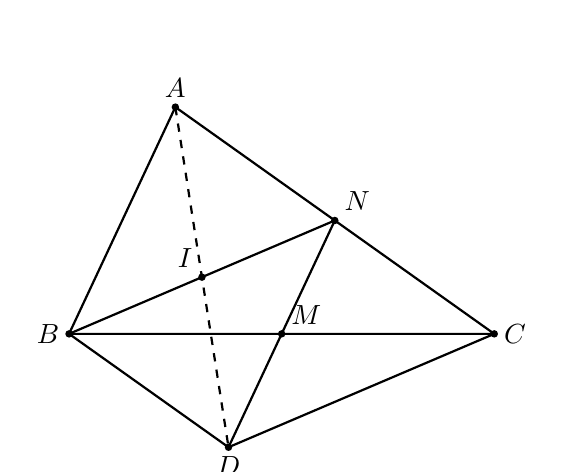
\begin{tikzpicture}[scale=0.9, >=stealth]
  \coordinate (B) at (0,0);
  \coordinate (C) at (6,0);
  \coordinate (A) at (1.5,3.2);
  \coordinate (M) at ($(B)!0.5!(C)$);
  \coordinate (N) at ($(A)!0.5!(C)$);
  \coordinate (D) at ($(M)!-1!(N)$);
  \coordinate (I) at ($(B)!0.5!(N)$);
  \draw[thick] (A)--(B)--(C)--cycle;
  \draw[thick] (B)--(D)--(C);
  \draw[thick] (N)--(D);
  \draw[thick, dashed] (A)--(D);
  \draw[thick] (B)--(N);
  \fill (A) circle (1.5pt) node[above] {$A$};
  \fill (B) circle (1.5pt) node[left] {$B$};
  \fill (C) circle (1.5pt) node[right] {$C$};
  \fill (M) circle (1.5pt) node[above right] {$M$};
  \fill (N) circle (1.5pt) node[above right] {$N$};
  \fill (D) circle (1.5pt) node[below] {$D$};
  \fill (I) circle (1.5pt) node[above left] {$I$};
\end{tikzpicture}
\end{center}
\begin{enumerate}[label=\textbf{\alph*)}, leftmargin=0.8cm, itemsep=0pt, topsep=1pt]
\item (0,5 điểm) Tứ giác $BNCD$ là hình gì? Vì sao?
\item (0,25 điểm) Gọi $I$ là trung điểm của $BN$. Chứng minh ba điểm $A, I, D$ thẳng hàng.
\item (0,25 điểm) Tìm điều kiện của tam giác $ABC$ để tứ giác $BNCD$ là hình thang cân.
\end{enumerate}
\loigiai{
\textbf{a)} \textit (0,5 điểm): Xét tứ giác $BNCD$, ta có $M$ là trung điểm của $BC$ (giả thiết) và $M$ là trung điểm của $ND$ (do $D$ thuộc tia đối của tia $MN$ và $MN = MD$). Tứ giác $BNCD$ có hai đường chéo $BC$ và $ND$ cắt nhau tại trung điểm $M$ của mỗi đường, do đó $BNCD$ là hình bình hành.

\textbf{b)} \textit (0,25 điểm): Trong tam giác $ABC$, $M$ và $N$ lần lượt là trung điểm của $BC$ và $AC$, do đó $MN$ là đường trung bình của tam giác $ABC$. Suy ra $MN \parallel AB$ và $MN = \dfrac{1}{2}AB$. Vì $D, M, N$ thẳng hàng và $DN = 2MN$, ta có $DN \parallel AB$ và $DN = AB$. Tứ giác $ABDN$ có cặp cạnh đối $DN$ song song và bằng $AB$ nên $ABDN$ là hình bình hành. Hai đường chéo $AD$ và $BN$ của hình bình hành $ABDN$ cắt nhau tại trung điểm mỗi đường. Do $I$ là trung điểm của $BN$ nên $I$ cũng là trung điểm của $AD$. Vậy ba điểm $A, I, D$ thẳng hàng.

\textbf{c)} \textit (0,25 điểm): Vì $BNCD$ là hình bình hành, để $BNCD$ là hình thang cân thì $BNCD$ phải là hình chữ nhật. Hình bình hành $BNCD$ là hình chữ nhật khi và chỉ khi $\widehat{BNC} = 90^\circ$, tức là $BN \perp AC$. Trong tam giác $ABC$, đường trung tuyến $BN$ đồng thời là đường cao khi và chỉ khi tam giác $ABC$ cân tại $B$. Vậy điều kiện cần tìm là tam giác $ABC$ cân tại $B$.


}
\end{ex}
\vspace{0.5mm}

\begin{ex} (0,5 điểm)
Tính nhanh giá trị biểu thức sau: $A = 8 \cdot (3^2 + 1)(3^4 + 1)(3^8 + 1)(3^{16} + 1)$.
\begin{enumerate}[label=\textbf{\alph*)}, leftmargin=0.8cm, itemsep=0pt, topsep=1pt]
\item (0,5 điểm) Tính nhanh giá trị của $A$.
\end{enumerate}
\loigiai{
\textbf{a)} \textit (0,5 điểm): Nhận xét: $8 = 3^2 - 1$. Thay vào biểu thức $A$, ta có:

$A = (3^2 - 1)(3^2 + 1)(3^4 + 1)(3^8 + 1)(3^{16} + 1)$

Áp dụng liên tiếp hằng đẳng thức hiệu hai bình phương $(a - b)(a + b) = a^2 - b^2$:

$= (3^4 - 1)(3^4 + 1)(3^8 + 1)(3^{16} + 1)$

$= (3^8 - 1)(3^8 + 1)(3^{16} + 1)$

$= (3^{16} - 1)(3^{16} + 1) = 3^{32} - 1$.

Vậy $A = 3^{32} - 1$.


}
\end{ex}
\vspace{0.5mm}


\enlargethispage{1.5cm}
\begin{center}
\rule{4cm}{0.4pt}\\
\textit{--- HẾT ---}
\end{center}
\end{document}
